\documentclass[myclassdoc,debug]{rjparticle}
%use the following command when typesetting your paper:
%\documentclass{rjparticle}
\usepackage{graphicx}

\title{Wobbling Nucleus I} 

\author[1,2,$a$]{R. Poenaru}
\author[2,3,$b$]{A. A. Raduta}

\affil[1]{Doctoral School of Physics, University of Bucharest, Bucharest, Romania\\
\email[a]{robert.poenaru@drd.unibuc.ro} }
\affil[2]{Department of Theoretical Physics - \textit{Horia Hulubei} National Institute for Physics and Nuclear Engineering, M\u{a}gurele-Bucharest, Romania\\
\email[b]{raduta@nipne.ro} (corresponding author)}
\affil[3]{Academy of Romanian Scientists, Bucharest, Romania}

\keywords{Nuclear Structure, Triaxial Nuclei, Wobbling Motion, Parity Symmetry, Signature Partners, Strong Deformation}

\pacs{01.30.-y, 01.30.Ww, 01.30.Xx, 99.00.Bogus}

\hyphenation{rjp-ar-ti-cle}

%%%%%%%%%%%%%%%%%%%%%%%%%%%%%%%%%%%%%%%%%%%%%%%%%%%%%%%%%%%%%%%%%%%%%%%%%%%%%%%
%Please, do not remove the following lines!
%%%%%%%%%%%%%%%%%%%%%%%%%%%%%%%%%%%%%%%%%%%%%%%%%%%%%%%%%%%%%%%%%%%%%%%%%%%%%%%
%\RJPVolume{63}{2018}
%\RJPNumber{1-2}
%\RJPPages{}{}
\columntitle{Wobbling Nucleus I}
%\date{}
%\dedication{}
%\domaintitle{}
%\keywords{}
%\pacs{01.30.-y, 01.30.Ww, 01.30.Xx, 99.00.Bogus}
%%%%%%%%%%%%%%%%%%%%%%%%%%%%%%%%%%%%%%%%%%%%%%%%%%%%%%%%%%%%%%%%%%%%%%%%%%%%%%%

\begin{document}
%%%%%%%%%%%%%%%%%%%%%%%%%%%%%%%%%%%%%%%%%%%%%%%%%%%%%%%%%%%%%%%%%%%%%%%%%%%%%%%
%Please, remove these lines when typesetting your document!
%%%%%%%%%%%%%%%%%%%%%%%%%%%%%%%%%%%%%%%%%%%%%%%%%%%%%%%%%%%%%%%%%%%%%%%%%%%%%%%
\lstset{%
basicstyle=\small,
language=[AlLaTeX]TeX,
columns=fullflexible,
%keepspaces=true,
showspaces=true,
showstringspaces=false,
keywordstyle=[2]\ttfamily,
identifierstyle=,
texcsstyle=*\ttfamily,
commentstyle=\color{gray},
string=[s]<>,
morestring=[b]',
stringstyle=\emph,
breaklines=true,
deletekeywords={list},
moretexcs={authnote,keywords,pacs},
}
%%%%%%%%%%%%%%%%%%%%%%%%%%%%%%%%%%%%%%%%%%%%%%%%%%%%%%%%%%%%%%%%%%%%%%%%%%%%%%%
\maketitle

\begin{abstract}
Abstract 1.
\end{abstract}

\section{Introduction}

Triaxiality in nuclei has become an interesting topic for physicists over the years, mainly due to the large number of characteristics that become apparent from these kinds of shapes but also for its great challenge of measuring it experimentally. Moreover, stable triaxial shapes are of rare occurrence across the chart of nuclides \cite{moller2006global}, since the predominant character of nuclei is either spherical or axially symmetric. Over the last two decades, it has been shown that triaxiality plays a crucial role in measurements of important quantities like separation energies of the nucleons \cite{moller2006global}, nucleon emission probabilities,  and also fission barriers in heavy nuclei  \cite{moller2009heavy}, however, concrete evidence of triaxiality in nuclei was still missing or under investigation. Tremendous work was made towards a clear signature for non-axially symmetric shapes: effects such as anomalous signature splitting \cite{hamamoto1988triaxial}, signature inversion \cite{bengtsson1984signature}, and staggering of $\gamma$ bands \cite{stachel1982triaxiality} were pointed out, but recently two clear fingerprints of nuclear triaxiality have emerged, based on both experimental and theoretical findings. Indeed, the phenomena of \emph{chiral symmetry breaking} \cite{frauendorf1997tilted} and that of \emph{wobbling motion} (W.M.) \cite{bohr1998nuclear} are considered as unique characteristics of nuclear triaxiality. 

The experimental observations regarding wobbling motion have been quite rare, even though this kind of collective motion has been theoretically predicted almost 50 years ago by Bohr and Mottelson \cite{bohr1998nuclear} when they were investigating the rotational modes of a triaxial nucleus employing a Triaxial Rotor Model (TRM). Therein, it was shown that for a triaxial rotor, the main rotational motion is around the axis with the largest moment of inertia (MOI), as it is energetically the most favorable. This mode is quantum-mechanically disturbed by the rotation around the other two axes, since rotation around any of the three principal axes of the system are possible, due to the anisotropy between the MOIs (that is $\mathcal{I}_1\neq\mathcal{I}_2\neq\mathcal{I}_3$). Naturally, the description of the energy spectra and electromagnetic transitions between the rotational states of these wobbling nuclei (also known as \emph{wobblers}) are considered to be the main characteristics that are put to the test by a theoretical investigation. The overall agreement between experimental results and the theoretically obtained data serves as an indicator for the quality of the model used to describe the wobbling picture.

The present work aims at extending the knowledge of the wobbling characteristics in an even-odd nucleus, which will be done by studying the energy spectrum of $^{163}$Lu in a semi-classical approach, where the rotational states are described through a set of classical equations. In contradistinction with previous work, \cite{raduta2020towards}, in this formalism, all four wobbling bands are described by the same \emph{core-quasiparticle alignment}, making thus the description of the wobbling motion consistent. A remarking feature for the current research is the introduction of the concept of \emph{parity partner bands} - concerning the states from $TSD_2$ and $TSD_4$ bands -  which will be discussed throughout the paper.

\section{\texorpdfstring{Re-interpretation of the wobbling bands in $^{163}$Lu}%
                               {Re-interpretation of the wobbling bands structure for 163Lu}}
\label{section-reinterpretation}

Considered the \emph{best wobbler} to date, $^{163}$Lu has a rich wobbling spectrum \cite{odegaard2001evidence,jensen2002evidence}, with no less than four such wobbling bands: one yrast - $TSD_1$, (zero-phonon wobbling number $n_w=0$), and three excited wobbling bands - $TSD_{2,3,4}$ (with their corresponding wobbling phonon numbers $n_w=1,2,3$). The name TSD comes from Triaxial Strongly Deformed bands. The triaxial bands emerge due to the coupling of an odd-$\vec{j}$ nucleon with an even-even triaxial core. Thus, for $^{163}$Lu, it is the intruder $\pi(i_{13/2})$ that couples to the triaxial core \cite{odegaard2001evidence,hamamoto2002wobbling,jensen2002wobbling}, driving the nuclear system up to large deformation, and stabilizing the deformed structure. Indeed, a triaxial shape with deformation parameters $(\epsilon_2,\gamma)\approx(0.38,+20^\circ)$ is assumed to be in agreement with the observed data, based on calculations using the Ultimate Cranker Code \cite{bengtsson1990high} for the potential energy surface (PES).

In terms of the experimental evidence which should be pointing out wobbling nature for the four TSD bands belonging to $^{163}$Lu, the large transition quadrupole moment $Q_t \approx 10\ b$ \cite{gorgen2004quadrupole}, the predominantly $E2$ character of the transitions linking adjacent bands ($I\to I-1$), a large $E2/M1$ mixing ratio $\delta>1$ for the transitions linking the yrare ($n_w=1$) and yrast ($n_w=0$) bands are all clear fingerprints of wobbling nature. For a set of results concerning these quantities (both theoretical and experimental), see Ref. \cite{raduta2017semiclassical}, and the references cited therein. Another quantity that indicates strong deformation with wobbling character is the relative rigid rotor energy, and for this isotope, calculations show that all four bands have similar behavior with respect to this value (see Figures 3 and 4 from Ref. \cite{hagemann2005triaxiality}).

Considering the experimental evidence which was indicated above and calculations based on particle rotor models, it can be summarized that the \emph{generally accepted} formalism for the band structure in $^{163}$Lu is the following:
\begin{itemize}
    \item There are three excited wobbling bands (w.b.) $TSD_2$, $TSD_3$, and $TSD_4$ and one ground-state w.b. $TSD_1$.
    \item The three excited w.b. have wobbling-phonon numbers $n_{w_2}=1$, $n_{w_3}=2$, and $n_{w_4}=3$, respectively.
    \item All three bands are built on top of the yrast state (the ground state band) with zero-wobbling-phonon number $n_{w_1}=0$.
    \item Stable triaxial super-deformation is achieved due to the alignment of the odd $\pi(i_{13/2})$ nucleon which couples to a triaxially deformed core $\vec{R}$.
    \item $TSD_{1,2,3}$ have all positive parity $\pi_1=\pi_2=\pi_3=+1$, while the spin states belonging to $TSD_4$ have negative parity $\pi_4=-1$. All states within the four bands have a half-integer spin.
 \end{itemize}

 In accordance with the band structure which was just formulated, a fully semi-classical approach for the description of the wobbling spectrum of $^{163}$Lu was by Raduta et. al. \cite{raduta2017semiclassical}. Therein, with the Time-Dependent Variational Equation (TDVE) applied on the PRM Hamiltonian and a trial wave-function that encapsulates both the states of the deformed nucleus $I$ and the single-particle states $j$, a set of analytical expressions for the excitation energies of all four bands was obtained. The energies belonging to the excited wobbling phonons were populated by the action of a phonon operator $\Gamma^\dagger$ on the ground state. Indeed, by acting with the phonon operator on the ground state with the spin $I=R+j$ and $R=0,2,4,\dots$, the states from $TSD_2$ ($n_w=1$) can be obtained. By applying twice ($n_w=2$) the phonon operator, the rotational states from $TSD_3$ will be created. Lastly, the states from $TSD_4$ are obtained with the action on the ground state with three ($n_w=3$) phonon operators: two of positive parity and one of negative parity (due to the overall negative parity $\pi_4=-1$ of $TSD_4$). One has to remark the fact that for $TSD_4$, the model assumes an odd-particle-rotor-coupling with a different intruder: the $\pi(h_{9/2})$ nucleon. This was suggested by the negative parity orbital which might be occupied by this proton, in the spherical shell model. Several calculations in the literature point out that this nucleon might be causing the third excited wobbling band to have negative parity \cite{jensen2004coexisting}. It is worthwhile mentioning that for the work described in \cite{raduta2017semiclassical}, the variational principle was only applied for the states in $TSD_1$ since the other three wobbling bands are obtained through phononic excitations via the phonon operator $\Gamma^\dagger$.

In what follows, it is useful to introduce some notations that will refer to the formalisms developed in the present paper and the one formulated in \cite{raduta2020towards} for the description of the wobbling motion in $^{163}$Lu. As such, the study developed in \cite{raduta2020towards} will be denoted with \texttt{W1}, while the current work will be shortly denoted by \texttt{W2}. For the sake of a self-consistent presentation, in subsection \ref{subsection:w1} a brief overview of the recently published work \texttt{W1} will be made, with further development of \texttt{W2} being presented in the subsection \ref{subsection:w2} - representing the \emph{core concept} of the current analysis.


\subsection{\texttt{W1} - Signature Partner Bands}
\label{subsection:w1}

Working with a semi-classical approach that is based on the triaxial particle rotor model, a full description of the wobbling bands for $^{163}$Lu was achieved, but with a slightly modified band structure. Indeed, rather than applying a TDVE just for the yrast $TSD_1$ band, the states from $TSD_2$ were also obtained variationally. This was possible due to the different coupling schemes that emerged for $TSD_1$ and $TSD_2$, respectively. More precisely, in \cite{raduta2020towards} and \cite{raduta2020approach} there are three different coupling schemes $(\vec{R}+\vec{j})$: states from $TSD_1$ arise from the odd $\pi(i_{13/2})$ intruder coupling with a core with angular momentum sequence $R_1=0,2,4,\dots$; states from $TSD_2$ arise from the same odd proton but coupling with a different triaxial core with angular momentum sequence $R_2=1,3,5,\dots$. The band $TSD_3$ is obtained as a set of states which are built on top of $TSD_2$, with the action of an $n_w=1$ wobbling quanta; this being different than the band structure previously mentioned were the third band was a two-phonon excitation of the yrast $TSD_1$. Lastly, the fourth band $TSD_4$ is a ground state band which results from the coupling of the same core as for $TSD_2$ (that is defined with the angular momentum sequence $R_2=1,3,5,\dots$) but with a different odd nucleon: $\pi(h_{9/2})$. Consequently, $TSD_2$ and $TSD_4$ are yrast states, alongside $TSD_1$.

For the first three bands, the MOIs are the same, and they are considered to be free parameters within the numerical calculations. However, this is not true for the fourth band, where a different set of MOIs had to be introduced, since for $TSD_4$ the core polarization effects are changed by coupling scheme.

%%%%%%%% UPDATE! %%%%%%%%
Using \texttt{W1}, the final results pointed out to the largest MOI corresponding to the 1-axis ($\mathcal{I}_1$ being the largest MOI obtained through the fitting procedure), making the system rotate around the 1-axis (that is the short $s$-axis). Moreover, the odd proton is aligned to the short axis as well, suggesting that the nucleus has an LW character. By representing the experimental wobbling energies according to Eq. \ref{wobbling-energy-relative}, it was obtained that both the theoretical, as well as the experimental values were increasing functions of angular momentum (keep in mind that the first wobbling band $n_w=1$ within the \texttt{W1} model is $TSD_3$). The agreement between the two sets of data (see Figure 6 from \cite{raduta2020approach}) indicates that the condition for LW/TW character of the wobbling bands stated by Frauendorf et. al. in \cite{frauendorf2014transverse} is not strictly related to the increasing/decreasing wobbling energy $E_\text{wob}$. In fact, referring to the case of the wobbling motion for $^{183}$Au, Nandi et. al. \cite{nandi2020first} also point out that the behavior of $E_\text{wob}$ under spin increase should not be the only indicator of a certain wobbling regime, since for a larger spin interval (if there is experimental data available) there could be regions with both increasing and decreasing trends in wobbling energy. There is an ongoing debate whether the behavior of an LW or TW triaxial nucleus is strictly related to the change in $E_{wob}$ with total a.m. \cite{tanabe2017stability,frauendorf2018comment,tanabe2018reply}.
%%%%%%%% UPDATE! %%%%%%%%

A final aspect that needs to be mentioned regarding \texttt{W1} has to do with the interpretation of $TSD_1$ and $TSD_2$ as being Signature Partner Bands (SPB). Signature \cite{bohr1998nuclear} is a quantum property that appears in deformed systems. It is strictly related to the invariance of a system with quadrupole deformation to a rotation by an angle $\pi$ around a principal axis. For example, a rotation around the $x$-axis will be defined as an operator:
\begin{align}
    \hat{R}_x=e^{i\pi\hat{I}_x}\ .
\end{align}

As for the framework used in \cite{raduta2020approach,raduta2020towards}, due to the wave-function describing the system being written as a product between the $\ket{I}$ basis state corresponding to the total angular momentum and the single-particle basis state $\ket{j}$, the rotation operator used in \texttt{W1} achieves the following form:
\begin{align}
    \hat{R}_x(\pi)=e^{-i\pi\hat{I}_x}\otimes e^{-i\pi\hat{j}_x}\ .
\end{align}

If the system has axial symmetry, only the rotation around any of the principal axes that are perpendicular to the symmetry one can define the signature quantum number. Consequently, the signature is a property specific to a deformed system and it translates to a so-called \emph{deformation invariance} with respect to space and time reflection properties \cite{bohr1998nuclear}. For an even-even nucleus, the signature operator $\hat{R}_x$ has two eigenvalues, -1 and 1. For the even-odd case, the eigenvalues are $-i$ and $+i$, and depending on the total spin, the signatures can have two values, given by the following assignment:
\begin{align}
    \alpha_I=\frac{1}{2}\left(-1\right)^{I-1/2}\ .
    \label{signature-formula-odd-nuclei}
\end{align}

Indeed, Eq. \ref{signature-formula-odd-nuclei} describes the signature quantum number for a state of angular momentum $I$ belonging to an odd mass nucleus. Such a rotational band with a sequence of states differing in spin by $\Delta I=1$ will be divided into two branches, each branch consisting of levels differing in spin by $\Delta I=2$, being related by the signature number $\alpha_I=\pm 1/2$. In \cite{raduta2020approach} the signature concept is brought to the classical picture associated with a triaxial nucleus employing rotation operators which act on the trial function (this function is a product of two coherent states, one that is associated to the core and one to the valence nucleon). Eqs. 27-29 from \cite{raduta2020approach} will extract two signatures for $TSD_1$ and $TSD_2$, namely the \emph{favored} signature $\alpha_{1f}=+1/2$ for the first band, and \emph{un-favored} signature $\alpha_{2u}=-1/2$ for the second band, respectively. A justification for the possibility of $TSD_1$ and $TSD_2$ of being SPB was based on the calculation of the triaxial potential (which was systematically performed in \cite{raduta2017semiclassical} and \cite{raduta2018wobbling}), concluding that the minimum is very deep, preventing in this way the states from $TSD_2$ to share other minima through tunneling effects. Other experimental and theoretical results \cite{sun1994varied,khalaf11properties,uma2015deltai,mittal2016signature} for deformed nuclei around this mass region suggest that the calculations performed in \texttt{W1} regarding the connection between $TSD_1$ and $TSD_2$ as belonging to a signature splitting phenomenon are valid and consistent with already existing interpretations.

It is instructive to mention a few key-points which arise based on the above discussion regarding \texttt{W1}:

\begin{enumerate}
    \item The wobbling band structure in $^{163}$Lu was re-interpreted: three bands are now yrast ground states, and only $TSD_3$ is one-phonon excited wobbling band (built on top of $TSD_2$)
    \item Both $TSD_1$ and $TSD_2$ are obtained variationally, by solving the time dependent variational equation associated to the initial quantal Hamiltonian
    \item There are three different $R+j$ coupling schemes that will produce the entire wobbling spectra of $^{163}$Lu (the following naming scheme is exclusive to this work):
    \begin{enumerate}
        \item Coupling $C_1$: The odd proton $j_1={13/2}$ is coupled to a core sequence with a.m. $R_1=0,2,4,\dots$ (even spin states for the triaxial rotor).
        \item Coupling $C_2$: The same odd proton $j_1={13/2}$ as in $C_1$ is coupled to a core sequence with a.m. $R_2=1,3,5,\dots$ (odd spin states for the triaxial rotor).
        \item Coupling $C_3$: A different odd proton $j_2={9/2}$ is coupled to the same core as in $C_2$.
    \end{enumerate}
    \item Two different sets of MOIs corresponding to the triaxial nucleus (that is the rotor coupled with the odd proton) are obtained as fitting parameters throughout the numerical calculations: one for the set $TSD_{1,2,3}$ and one for $TSD_4$.
    \item $TSD_1$ and $TSD_2$ are Signature Partner Bands: with $TSD_1$ ($TSD_2$) being the favored (un-favored) partner. Their corresponding signature quantum numbers are $\alpha_{1f}=+1/2$ and $\alpha_{2u}=-1/2$.
    \item As a side-by-side comparison with regards to the overall agreement with the experimental data, \texttt{W1} yielded better results when compared to the previous work depicted in Ref. \cite{raduta2007semiclassical}, although it must be mentioned that both models are based on semi-classical approaches.
\end{enumerate}

A diagram that shows the workflow involved in \texttt{W1} can be seen in Figure \ref{w1-model-worfklow} from the Appendix. Also, a comparison with previous calculations can be seen in Figure 21 from Ref. \cite{raduta2020approach}.

\subsection{\texttt{W2} - Signature Partner Bands + Parity Partner Bands}
\label{subsection:w2}

The main question which can be asked regarding the formalism \texttt{W1} that was described in \ref{subsection:w1} is whether it is possible to obtain a \emph{unified} description for all four bands in $^{163}$Lu concerning the coupling scheme. In other words, it is worth investigating the possibility of having a unique single-particle state $j$ that is coupled to a core of positive parity for the bands $TSD_{1,2,3}$ and a core of negative parity for $TSD_4$.

Fortunately, the answer is positive: starting from the semi-classical formalism of \texttt{W1}, one can properly adjust the coupling scheme, making sure that the entire numerical recipe used for obtaining the energy spectrum of $^{163}$Lu remains consistent with the experimental results.

Regarding the unique single-particle that couples to the triaxial core, it is natural to pick the $i_{13/2}$ proton (that is $j_1$ from \texttt{W1}). The reasoning behind this choice has to do with the microscopic calculations \cite{jensen2002wobbling,hagemann2003quantized,jensen2004coexisting} that showed stable triaxial structures in the $^{163}$Lu potential energy surface when the triaxial core couples with a highly aligned $j$-shell particle, indicating the $\pi(i_{13/2})$ proton. Keep in mind that a highly aligned $j$-nucleon will \emph{prefer} to keep a certain triaxial deformation when coupled to a core \cite{hamamoto1983intrinsic,hamamoto1987rotational,hamamoto2016interplay} (in the sense that the triaxiality parameter $\gamma$ will have a certain value based on the orbital of the odd nucleon), and using microscopic calculations following the Ultimate Cranker code, it has been shown that a value of $\gamma\approx+20^\circ$ is preferred by the odd $\pi(i_{13/2})$ nucleon.

By taking $j=j_1$ as the sole intruder that couples to a positive core and also a negative core, the sequences with even/odd integer spins for the core do not change. In fact, the coupling schemes can be readily obtained:

\begin{enumerate}
    \item Coupling $C'_1$: the odd $j_1$ proton aligns with the core of even-integer spin sequence $R_1=0,2,4,\dots$, with a parity of the $R_1$ core that is positive $\pi(R_1)=+1$.
    \item Coupling $C'_2$: the odd $j_1$ proton aligns with the core of even-integer spin sequence $R_2^+=1,3,5,\dots$, with a parity of the $R_2^+$ core that is positive $\pi(R_2^+)=+1$.
    \item Coupling $C'_3$: the odd $j_1$ proton aligns with the core with an odd-integer spin sequence $R_2^-=1,3,5,\dots$, which has negative parity $\pi(R_2^-)=-1$.
\end{enumerate}

From the three schemes defined above, it is clear that $C'_1$ corresponds to the yrast $TSD_1$, $C'_2$ to the ground state $TSD_2$, and finally $C'_3$ to the ground state $TSD_4$. Obviously, the odd valence nucleon $j_1$ has a positive parity $\pi_{j_1}=+1$. There has not been attributed a coupling scheme for $TSD_3$, since this band still remains as the one-wobbling phonon excitation that is built on top of $TSD_2$ with the action of a phonon operator which will be characterized later on. The three couplings are schematically represented in Figure \ref{three-couplings}. One should keep in mind the fact that $\vec{j}$ is aligned with the axis with the largest MOI does not necessarily mean the fact that the model works within the Frozen Alignment approximation - it is just an illustration.

\begin{figure}
    \centering
    % 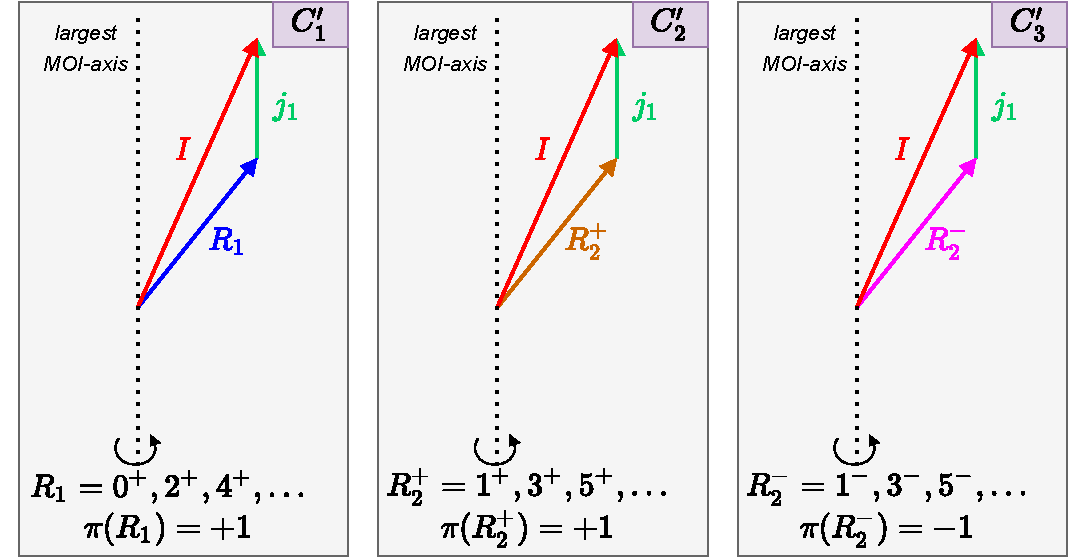
\includegraphics[width=0.95\textwidth]{figs/coupling_schemes_C1C2C3.pdf}
    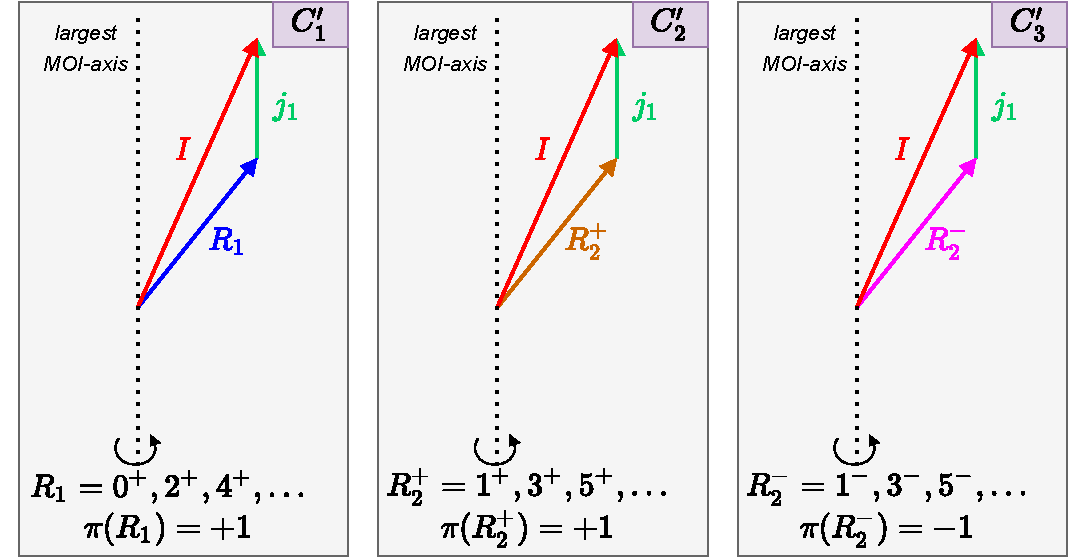
\includegraphics[scale=0.7]{figs/coupling_schemes_C1C2C3.pdf}
    \caption{A schematic representation with the three coupling schemes that characterize the \texttt{W2} model. The same odd particle ($j_1=i_{13/2}$ proton) is coupled with two positive cores with even (odd) integer spin sequences for $TSD_1$ ($TSD_2$), and one negative core in the case of $TSD_4$ with odd integer spin sequence. The total spin of the system precesses around the axis with the largest MOI, as it is the case for a triaxial rotor.}
    \label{three-couplings}
\end{figure}

The last step in searching for a unified coupling scheme in $^{163}$Lu is to establish a possible relationship between the four bands. As per the calculations involved in \texttt{W1}, it was proven that signature is a good quantum number and indeed, a sign that $TSD_1$ and $TSD_2$ are signature partners emerged. Their overall similar properties and spin difference enforce this argument. Furthermore, in this new \texttt{W2} approach, the difference in parity between the $TSD_2$ and $TSD_4$ but the same angular momentum sequence of their corresponding triaxial core $R_2^+$ and $R_2^-$ strongly suggest that the two bands are \emph{Parity Partner Bands}: two rotational sequences with energy states characterized by opposite parity, increasing energy that follows a trend $\propto I(I+1)$, and a spin difference $\Delta I=2$ between states belonging to the same band. In the following section, calculations which will show that parity is indeed a good quantum number for the triaxial rotor + odd-particle system will be provided. For what it is worth mentioning now is that the concept of parity partners between $TSD_2$ and $TSD_4$ emerge from the idea that a stable strongly deformed structure is achieved from a single quasiparticle that moves in a quadrupole mean-field generated by a triaxial even-even core. However, there is a splitting in two different cases of coupling mechanisms, namely $C'_2$/$C'_3$ depending on the alignment of the high-$j$-shell particle with a core of positive/negative parity.

Similar structures with alternating positive-negative parity bands have been also reported in other nuclei such as $^{40}$Ca \cite{torilov2004spectroscopy}, or some heavier isotopes like $^{218}$Fr \cite{debray2000alternating}. In fact, a unified description of states with positive and negative parity in odd-mass nuclei was made over the last decade \cite{radutaa2009csm,raduta2011simultaneous}, although therein, a quadrupole-octupole term was introduced within the particle-core Hamiltonian to describe this feature. A diagram which shows the workflow involved in \texttt{W2} can be seen in the Figure \ref{w2-model-worfklow} from the Appendix \ref{appendix:a}.


\section{Examples for various Environments}
This section includes examples of different environments containing media and data material (the copyright of which is already owned by RJP) much needed in any good scientific publication. For instance below (in figure \ref{pic1}) we present a \textit{figure} environment as it must appear in every contribution submitted to our journal (this picture is in PNG format so compiling must be done using \textit{pdflatex} command rather than the usual \textit{latex} command or one should specify the \textbf{pdftex} driver when loading the \textbf{graphicx} package).
\begin{figure}[h!tb]
\centering
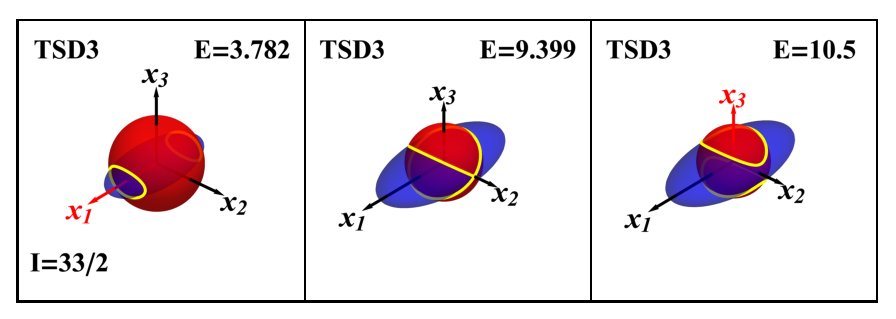
\includegraphics[width=0.8\textwidth]{tsd3_spin1.eps}
\caption{This is a sample picture taken from RJP volume \textbf{50}(1-2) from page 129 (2005).It illustrates (hashed areas) the instability domains for a series of nonlinear Schr\"odinger equations determined using the deterministic approach to modulational instability.}
\label{pic1}
\end{figure}


\section{Theoretical Formalism}
\label{section-theory}

In this section, a description of the framework used for obtaining the wobbling spectrum of $^{163}$Lu is made. As stated in the previous section, the system is described with a similar Hamiltonian used in \texttt{W1}, namely the Hamiltonian for the triaxial PRM.
\begin{align}
    H=H_\text{core}+H_\text{s.p.}\ .
    \label{prm-hamiltonian}
\end{align}

The Hamiltonian from Eq. \ref{prm-hamiltonian} describes a system in which an odd $j$ particle interacts with a triaxial even-even core i.e., the odd nucleon is moving in a quadrupole deformed mean-field that is generated by the core. As such, the first term in the Hamiltonian $H_\text{core}$ describes the motion of a triaxial core, while the second term $H_\text{s.p.}$ represents the single-particle potential characterizing the valence proton.

Indeed, the core Hamiltonian is given by:
\begin{align}
    H_\text{core}=\sum_{i=1,2,3}\frac{1}{2\mathcal{I}_i}(I_i-j_i)^2\ ,
    \label{core-hamiltonian}
\end{align}
where the core angular momentum is $\vec{R}=\vec{I}-\vec{j}$ and the terms $\mathcal{I}_i$ represent the moments of inertia for a triaxial ellipsoid, along the principal axes. These three moments of inertia will be considered as free parameters in the present calculations, but, compared to the work \texttt{W1}, a unique set of MOIs will be attributed to the four bands, since the triaxial core will create an alignment with a unique particle, that is $j_1$. Because of this, there is no option for their nature (i.e., rigid or hydrodynamic).

The single-particle Hamiltonian from Eq. \ref{prm-hamiltonian} is derived from the well-known Nilsson potential \cite{meyer1975collective,wang2008description}:
\begin{align}
    h(\beta_2,\gamma)=C\left\{\cos\gamma Y_{20}(\theta,\varphi)+\frac{\sin\gamma}{\sqrt{2}}\left[Y_{22}(\theta,\varphi)+Y_{2-2}(\theta,\varphi)\right]\right\}\ ,
    \label{nilsson-potential}
\end{align}
where the coupling parameter $C$ causes the level splitting in the deformed field and it is proportional to the quadrupole deformation $\beta_2$. The potential $h$ from Eq. \ref{nilsson-potential} is written in terms of the quadrupole deformation and triaxiality parameter that play the role of deformation parameters within a triaxial system $(\beta_2,\gamma)$. Its expression using the coupling parameter $C$ is widely used when working with a particle-rotor-model \cite{peng2003description,koike2004chiral,wang2007doublet}. In the present this case, the change $h(\beta_2,\gamma)\to H_\text{s.p.}$ is done by applying the Wigner-Eckart theorem for the single-$j$ particle, and the following expression for $H_\text{s.p.}$ will be obtained:
\begin{align}
    H_\text{s.p.}=\frac{V}{j(j+1)}\left[\cos\gamma(3j_3^2-\vec{j}^2)-\sqrt{3}\sin\gamma(j_1^2-j_2^2)\right]+\epsilon_j\ .
    \label{single-particle-hamiltonian}
\end{align}

This term describes the motion of an odd particle with angular momentum $j$ in a mean-field generated by a triaxial core, with a potential strength $V$ characterized by the quadrupole deformation ($V\propto\beta_2)$. In fact, the single-particle potential strength $V$ will be considered as the fourth free parameter within the calculations and its behavior will dictate the coupling of the $j$ particle with all four TSD bands. The term $\epsilon_j$ from Eq. \ref{single-particle-hamiltonian} represents the single-particle energy that corresponds to the odd $j$ proton from the $i$-orbital. One should not mix up the $j_1$ proton notation used throughout the paper with the components of the single-particle angular momentum from  Eq. \ref{single-particle-hamiltonian}.

Regarding the triaxial deformation $\gamma$ which enters in Eq. \ref{single-particle-hamiltonian}, its value will be considered as another free parameter of the current problem. In other words, having $V$ and $\gamma$ as free parameters means that the system will be described by its deformation parameters which will be obtained through a fitting procedure, keeping an agreement with the experimental data regarding the excitation energies of the rotational states belonging to $TSD_{1,2,3,4}$.

From Eqs. \ref{core-hamiltonian} and \ref{single-particle-hamiltonian}, the free parameter set can be obtained, hereafter denoted by $\mathcal{P}$. It comprises three moments of inertia, the single-particle potential strength, and the triaxial deformation. As such, $\mathcal{P}$ can be written as:
\begin{align}
    \mathcal{P}=\left[\mathcal{I}_1,\mathcal{I}_2,\mathcal{I}_3,V,\gamma\right]\ .
    \label{parameter-set}
\end{align}

Solving the problem of \texttt{W2} is equivalent to finding the eigenvalues of $H$ given in Eq. \ref{prm-hamiltonian}. In a similar approach as in \texttt{W1}, the eigenvalues of interest are obtained on the base of a semi-classical approach. Thus, the first step is to perform a de-quantization procedure on $H$ through a TDVE \cite{raduta2007semiclassical,budaca2018tilted,raduta2017semiclassical}:
\begin{align}
    \delta\int_0^t\bra{\Psi_{IjM}}H-i\frac{\partial}{\partial t'}\ket{\Psi_{IjM}}dt'=0\ .
    \label{tdve}
\end{align}

Working within a semi-classical approach allows one to keep close contact with the system's dynamics in terms of equations of motion for the generalized coordinates. The trial function from Eq. \ref{tdve} is carefully chosen as a product of two basis states comprising the states with total angular momentum $I$ and $j$, respectively:
\begin{align}
    \ket{\Psi_{IjM}}=\mathbf{N}e^{z\hat{I}_-}e^{s\hat{j}_-}\ket{IMI}\ket{jj}\ ,
    \label{trial-function}
\end{align}
where the operators $\hat{I}_-$ and $\hat{j}_-$ denote the lowering operators for the intrinsic angular momenta $\vec{I}$ and $\vec{j}$, respectively, and $\mathbf{N}$ plays the role of the normalization constant. One must remark the fact that the states $\ket{IMI}$ and $\ket{jj}$ from Eq. \ref{trial-function} are extremal states for the operators $(\hat{I}^2,\hat{I}_3)$ and $(\hat{j^2},\hat{j_3})$, respectively, and they correspond to the maximally allowed states for a given set of angular momenta $I$ and $j$. As an observation, the trial function is an admixture of components of definite $K$, which is consistent with the fact that for a triaxial nucleus, $K$ is not a good quantum number.

The variables $z$ and $s$ from Eq. \ref{trial-function} are complex functions of time, and they play the role of classical coordinates in the phase spaces that describe the motion of the core and the odd particle:
\begin{align}
    z=\rho e^{i\varphi}\ ,\ s=fe^{i\psi}\ .
    \label{complex-variable-set}
\end{align}

In order to obtain a set of classical equations in a Hamilton Canonical form, a new pair of variables are introduced: 
\begin{align}
    r=\frac{2I}{1+\rho^2}\ ,\ t=\frac{2j}{1+f^2}\ ,
\end{align}
where $r\in\left[0,2I\right]$ and $t\in\left[0,2j\right]$.Thus the equations of motion acquire the form:
\begin{align}
    \frac{\partial\mathcal{H}}{\partial r}&=\dot{\varphi}\ ;\ \frac{\partial\mathcal{H}}{\partial \varphi}=-\dot{r}\ , \nonumber\\
    \frac{\partial\mathcal{H}}{\partial t}&=\dot{\psi}\ ;\ \frac{\partial\mathcal{H}}{\partial \psi}=-\dot{t}\ .
    \label{eq-motion}
\end{align}

The function $\mathcal{H}$ denotes the average of the Hamiltonian operator $H$ (Eq. \ref{prm-hamiltonian}) with the trial function $\ket{\Psi_{IjM}}$ given in Eq. \ref{trial-function}, and it plays the role of classical energy:
\begin{align}
    \mathcal{H}(\varphi,r;\psi,t)=\bra{\Psi_{IjM}}H\ket{\Psi_{IjM}}\ ,
\end{align}

Starting from the equations of motion given in Eq. \ref{eq-motion}, one can observe that the function $\mathcal{H}$ is a constant of motion, that is $\dot{\mathcal{H}}\equiv0$. This equation will define a surface, a so-called equi-energy surface $\mathcal{H}=\text{const}$. It is worth mentioning the fact that such equality holds since the entire set of equations of motion emerged from a variational principle. The sign of the Hessian associated to this classical function will indicate its stationary points. Among them, some are minima. The critical points which are of interest for the present study are those obtained when the following ordering for the three moments of inertia holds: $\mathcal{I}_1>\mathcal{I}_2>\mathcal{I}_3$. There is no restriction on $\gamma$.

With a linearization procedure for the equations of motion around the minimum point  of $\mathcal{H}$, a dispersion equation will be obtained:
\begin{align}
    \Omega^4+B\Omega^2+C=0\ .
    \label{dispersion-eq}
\end{align}

The above equation describes a harmonic type of motion for the nuclear system, with the solutions to this algebraic equation as the \emph{wobbling frequencies} $\Omega$. The terms $B$ and $C$ are  functions of total angular momentum $I$, single-particle a.m. $j$, inertial parameters $A_k=1/(2\mathcal{I}_k)\ ,\ k=1,2,3$, single-particle potential strength $V$, and triaxiality parameter $\gamma$.  The $B$ term from Eq. \ref{dispersion-eq} has the expression \cite{raduta2020approach}:
\begin{align}
 -B=\left[(2I-1)(A_3-A_1)+2jA_1\right]\left[(2I-1)(A_2-A_1)+2jA_1\right]+8A_2A_3Ij+\text{T}_B^1\text{T}_B^2\ ,
 \label{b_term}
 \end{align}
 where the terms $\text{T}_B^1$ and $\text{T}_B^2$ are defined defined as:
 \begin{align}
 \text{T}_B^1&=\left[(2j-1)(A_3-A_1)+2IA_1+V\frac{2j-1}{j(j+1)}\sqrt{3}(\sqrt{3}\cos\gamma+\sin\gamma)\right]\ , \nonumber \\
 \text{T}_B^2&=\left[(2j-1)(A_2-A_1)+2IA_1+V\frac{2j-1}{j(j+1)}2\sqrt{3}\sin\gamma\right]\ .
 \label{b_term-plus}
\end{align}

Accordingly, the $C$ term from Eq. \ref{dispersion-eq} has the expression \cite{raduta2020approach}:
\begin{align}
    C=&\left\{\left[(2I-1)(A_3-A_1)+2jA_1\right]\text{T}_C^1
- 4IjA_3^2\right \} \nonumber\\
      &\times\left\{\left[(2I-1)(A_2-A_1)+2jA_1\right]\text{T}_C^2-4IjA_2^2\right\}\ ,
      \label{c_term}
\end{align}
where the terms $\text{T}_C^1$ and $\text{T}_C^2$ are defined defined as:
\begin{align}
    \text{T}_C^1&=\left[(2j-1)(A_3-A_1)+2IA_1+V\frac{2j-1}{j(j+1)}\sqrt{3}(\sqrt{3}\cos\gamma+\sin\gamma)\right]\ , \nonumber\\
    \text{T}_C^2&=\left[(2j-1)(A_2-A_1)+2IA_1+V\frac{2j-1}{j(j+1)}2\sqrt{3}\sin\gamma\right]\ . 
    \label{c_term-plus}
\end{align}

It can be seen that the terms which enter in $B$ and $C$, namely $(\text{T}_B^1,\text{T}_B^2)$ from Eq. \ref{b_term-plus} and $(\text{T}_C^1,\text{T}_C^2)$ from Eq. \ref{c_term-plus} correspond to the quadrupole deformation that causes the single-particle to move in the mean-field of the triaxial core. The terms also define the triaxiality that the nucleus achieves once the odd proton couples to the triaxial core, driving the system up to a large (and stable) deformation.

Going back to Eq. \ref{dispersion-eq}, under the restrictions for the MOIs defined above, the dispersion equation admits two real and positive solutions (hereafter denoted with $\Omega_1^I$ and $\Omega_2^I$, where $\Omega_1^I<\Omega_2^I$) defined for $j_1=i_{13/2}$, given by:
\begin{align}
    \Omega_{1,2}^I=\sqrt{\frac{1}{2}\left(-B\mp(B^2-4C)^{1/2}\right)}\ .
    \label{wobbling-frequencies}
\end{align}

These two solutions are interpreted as \emph{wobbling frequencies} associated with the motion of the core, and the motion of the odd-particle respectively. As such, each wobbling frequency has an associated wobbling-phonon number:
\begin{align}
    \Omega_1^I \to n_{w_1}\ ;\ \Omega_2^I \to n_{w_2}\ .
\end{align}


Now  the analytical expressions for the four TSD bands in $^{163}$Lu are readily obtained:
\begin{align}
    E_\text{TSD1}^I&=\epsilon_j+\mathcal{H}_\text{min}^{(I,j)}+\mathcal{F}_{00}^I\ ,\ I=13/2,17/2,21/2\dots \nonumber \\
    E_\text{TSD2}^I&=\epsilon_j^1+\mathcal{H}_\text{min}^{(I,j)}+\mathcal{F}_{00}^I\ ,\ I=27/2,31/2,35/2\dots \nonumber \\
    E_\text{TSD3}^I&=\epsilon_j+\mathcal{H}_\text{min}^{(I-1,j)}+\mathcal{F}_{10}^{I-1}\ ,\ I=33/2,37/2,41/2\dots \nonumber \\
    E_\text{TSD4}^I&=\epsilon_j^2+\mathcal{H}_\text{min}^{(I,j)}+\mathcal{F}_{00}^I\ ,\ I=47/2,51/2,55/2\dots\ ,
    \label{wobbling_energies}
\end{align}
where $\mathcal{F}_{n_{w_1}n_{w_2}}^I$ is a function of the wobbling frequencies:
\begin{align}
    \mathcal{F}_{n_{w_1}n_{w_2}}^I=\Omega_1^I\left(n_{w_1}+\frac{1}{2}\right)+\Omega_2^I\left(n_{w_2}+\frac{1}{2}\right)\ ,
    \label{f-term}
\end{align}
and $\mathcal{H}_\text{min}^{(I,j)}$ is the classical energy evaluated in its minimal point. For the present case, its analytical expression is given by the following equation:
\begin{align}
\mathcal{H}_\text{min}^{(I,j)}=(A_2+A_3)\frac{I+j}{2}+A_1(I-j)^2-V\frac{2j-1}{j+1}\sin\left(\gamma+\frac{\pi}{6}\right)\ .
    \label{hmin:equation}
\end{align}

A few aspects regarding the energy spectrum defined in Eq. \ref{wobbling_energies} are worth mentioning. To each band, there is a specific energy $\epsilon_j$ associated with the single-particle state. In this case, the odd-proton $j_1=13/2$ from the $i$-orbital is the one that couples to the triaxial core. However, for the bands $TSD_2$ and $TSD_4$, a different re-normalization of $\epsilon_j$ is considered, since $TSD_2$ is the unfavored signature partner of $TSD_1$, and $TSD_4$ is the negative parity partner of $TSD_2$ within the band structure. These quantities will shift the overall energy states belonging to the two bands, each by a different amount. As a result, both $\epsilon_j^1$ and $\epsilon_j^2$ will be adjusted throughout the numerical calculations such that the energy spectrum is best reproduced. Another aspect concerns the band $TSD_3$; since this is the only excited wobbling band within the family, its configuration is built on top of $TSD_2$, with the action of a single phonon ($n_{w_1}=1$) operator. Consequently, an energy state $I$ belonging to $TSD_3$ is obtained from a state $I-1$ from $TSD_2$. In Table \ref{energy-states-tabular}, the rest of the wobbling phonon numbers are mentioned, with the parity, signature, and coupling scheme for each band in particular.

\begin{table}
\centering
\begin{tabular}{llllll}
\hline
Band & $n_{w_1}$ & $n_{w_2}$ & $\pi$ & $\alpha$ & Coupling scheme\\
\hline
\hline
   $TSD_1$  &   0        &    0       & +1      &    +1/2      &   $C'_1$              \\
   $TSD_2$  &     0      &      0     &   +1    &  -1/2        &   $C'_2$              \\
   $TSD_3$  &   1        &      0     &     +1  &     +1/2    &  Built on top of $TSD_2$                \\
   $TSD_4$  &    0       &      0     &      -1 &   -1/2       &    $C'_3$    \\       
   \hline
\end{tabular}
\caption{The wobbling phonon numbers, parities, signatures, and coupling schemes assigned to each triaxial band in $^{163}$Lu, within the \texttt{W2} model. The three coupling schemes were defined in Section \ref{subsection:w2}.}
\label{energy-states-tabular}
\end{table}

\subsection{Parity quantum number for the wave-function}

In \texttt{W1} it was shown that signature emerges from the calculations on the total wave-function as a good quantum number for this triaxial system. This is why in \cite{raduta2020approach} the bands $TSD_1$ and $TSD_2$ appeared as Signature Partner Bands (SPB). In \texttt{W2}, such property still stands.

Since the backbone of the current work started from the need for a single odd-particle that couples to a triaxial core in $^{163}$Lu, one has to look at the band $TSD_4$ (which was interpreted as having a different nucleon: $j_2$ with $j=9/2$ from the $h$-orbital), and see if its differentiating properties can be linked to \emph{main group} of bands (namely $TSD_{1,2,3}$). Indeed, from the experimental measurements regarding spin and parity assignment \cite{jensen2004coexisting}, it turns out that the parity of the rotational states is negative. Therefore, a forensic analysis on this quantum property should be considered as the necessary ingredient in a unified description of all four bands.

 The parity operator is defined as a product of the complex conjugation operation and a rotation of angle $\pi$ around the 2-axis: $P=e^{-i\pi\hat{I}_2}C$. The total parity operator is the product of an operator corresponding to the core and one corresponding to the single-particle:
\begin{align}
    \mathcal{P}_T=P_\text{core}P_\text{s.p.}\ .
    \label{parity-operator}
\end{align}

Acting with the total parity operator defined above, on the trial function $\Psi$ associated , the following result is obtained:
\begin{align}
    \mathcal{P}_T\Psi(r,\varphi;t,\psi)=\Psi(r,\varphi+\pi;t,\psi+\pi)\overset{\mathrm{not.}}{=}\ \bar{\Psi}.
    \label{parity-action}
\end{align}

The classical energy function $\mathcal{H}$ has an invariance property at changing the angles with $\pi$:
\begin{align}
    \mathcal{H}(r,\varphi;t,\psi)=\mathcal{H}(r,\varphi+\pi;t,\psi+\pi)\ .
    \label{classical-energy-invariance}
\end{align}

From Eqs. \ref{parity-action} and \ref{classical-energy-invariance}, it can be concluded that the wave-function describing the triaxial system $\Psi$ and its image through $\mathcal{P}_T$ , $\bar{\Psi}$,  are two linearly dependent functions which differ only by a multiplicative constant $p$, with $|p|=1$. Thus, $p$ can either be -1 or +1, such that:
\begin{align}
    % \Psi(r,\varphi+\pi;t,\psi+\pi)=\pm\Psi(r,\varphi;t,\psi)\ .
    \bar{\Psi}=\pm\Psi(r,\varphi;t,\psi)\ .
\end{align}

The above result concludes the parity analysis for the wave-function, showing that the triaxial rotor admits eigenfunctions of negative parity. Therefore, a single wave-function characterized by the coupling of a triaxial core to the odd proton $i_{13/2}$ is describing both positive parity states ($\in TSD_{1,2,3}$) as well as negative parity states ($\in TSD_4$). This analysis, together with the fact that $TSD_2$ and $TSD_4$ have the same a.m. sequences (although $TSD_2$ has more states with low spin than $TSD_4$) suggest the fact that these two bands might be Parity Partners.


\section{Numerical results}
\label{section-results}

As a first step, the results concerning the excited spectrum of the four TSD bands will be presented. Regarding the wobbling spectrum of $^{163}$Lu, its analytical formulation was given in Eq. \ref{wobbling_energies}. As mentioned, those energies are parametrized in terms of $\mathcal{P}$, which is the set of free parameters to be determined. Indeed, one can find $\mathcal{P}$ by minimizing the $\chi^2$ function:
\begin{align}
    \chi^2=\frac{1}{N_T}\sum_{i}\frac{(E^{(i)}_\text{exp}-E^{(i)}_\text{th})^2}{E^{(i)}_\text{exp}}\ ,
    \label{chi-square}
\end{align}
where $N_T$ represents the total number of states. Table \ref{4-band-information} contains the number of states within each band, with the spin sequences for the core ($\vec{R}$), the spin sequences for the coupled system (that is the total angular momentum $\vec{I})$, and the coupling schemes specific to \texttt{W2} formalism that is used in the current calculations. 

\begin{table}
    \centering
  \begin{tabular}{llllll}
  \hline
  Band & $n_s$ & $\vec{j}$ & $\vec{R}$ - Sequence & $\vec{I}$ - Sequence & Coupling scheme \\
  \hline
  \hline
     $TSD_1$ &       21      &   $j_1$  &        $R_1=0,2,4,\dots$         &   $13/2,17/2,21/2,\dots$    & $C'_1$     \\
     $TSD_2$ &        17     &   $j_1$   &       $R_2^+=1^+,3^+,5^+,\dots$             &      $27/2,31/2,35/2,\dots$                &      $C'_2$           \\
     $TSD_3$ &      14       &    $j_1$  &           1-phonon excitation         & $33/2,37/2,41/2,\dots$                &       1-phonon excitation           \\
     $TSD_4$ &       11      &   $j_1$   &    $R_2^-=1^-,3^-,5^-,\dots$                &               $47/2,51/2,55/2,\dots$         &      $C'_3$          \\
     \hline
\end{tabular}
    \caption{The number of energy states $n_s$ within each wobbling band, the a.m. of the proton $\vec{j}$, the core's a.m. $\vec{R}$, the nucleus' a.m. $\vec{I}$, and the corresponding coupling scheme that was established according to the \texttt{W2} model. The single-particle is the $j_1=(i_{13/2})$ proton.}
    \label{4-band-information}
\end{table}

The resulting values for $\mathcal{P}$ are given  in Table \ref{parameter_set}. This \texttt{W2} method contrasts the approach in \texttt{W1}, where a second minimization process was needed separately for $TSD_4$. The root mean square error provided by the obtained parameter set $\mathcal{P}$ has a value of $E_\text{rms}\approx 79\ \text{keV}$. This result is much better than the one obtained with previous formalism \texttt{W1} where an $E_\text{rms}\approx240\ \text{keV}$ was obtained \cite{raduta2020approach}). As a matter of fact, this is the first semi-classical formalism in the literature that achieves agreement with the experimental data with less than $100\ \text{keV}$ for the entire wobbling spectrum of $^{163}$Lu. It is worth mentioning that the fitting procedure was done not for the absolute wobbling energies $E_\text{TSDk}^I\ ,\ k=1,2,3,4$, but for the \emph{excitation energies} which are relative to the hand-head $I=13/2^+$ from the first yrast band $TSD_1$. Comparison between the theoretical values obtained within the current formalism and the experimental data is shown in Figures \ref{energies-tsd12} and \ref{energies-tsd34}. For the sake of completeness, the wobbling frequencies which enter in the expression of the $\mathcal{F}_{n_{w_1}n_{w_2}}^I$ given by Eq. \ref{f-term} are graphically represented as functions of total angular momentum $I$ in Figure \ref{hydro-mois}, for the fixed parameter set. It is remarkable the fact that the wobbling frequency $\Omega_2^I$ is much larger than its partner, suggesting the fact the coupling effects caused by the highly aligned proton have a stronger influence in achieving a wobbling character for $^{163}$Lu, which is in line with the characteristics of a particle-rotor coupling. Another feature of these wobbling frequencies is their linear behavior with respect to the nuclear spin.

\begin{table}
    \centering
  \begin{tabular}{lllll}
  \hline
$\mathcal{I}_1$ [$\hbar^2$/\text{MeV}] & $\mathcal{I}_2$ [$\hbar^2$/\text{MeV}]& $\mathcal{I}_3$ [$\hbar^2$/\text{MeV}] & $\gamma$ [deg. ] & $V$ [\text{MeV}] \\
\hline
\hline
72              & 15              & 7               & 22       & 2.1\\
\hline
\end{tabular}
    \caption{The parameter set $\mathcal{P}$ that was determined by a fitting procedure of the excitation energies for $^{163}$Lu. }
    \label{parameter_set}
\end{table}

Concerning the single-particle energies from Eq. \ref{wobbling_energies}, namely $\epsilon_j^1$ and $\epsilon_j^2$ that emerge from the un-favored signature of $TSD_2$ and negative parity of $TSD_4$, respectively, they induce a correction for the mean-field with the quantities $\epsilon_j^1-\epsilon_j=0.3\ \text{MeV}$ and $\epsilon_j^2-\epsilon_j=0.6\ \text{MeV}$. Note that since the energy state $I_{13/2}\in TSD_1$ (the band-head of $TSD_1$) was subtracted from all bands, the single-particle energies for band 2 and 4 are adjusted accordingly.

The quantity $\epsilon_j^1-e_j$ is added to the second band due to the core, and such a splitting is caused by the fact that two distinct TDVE procedures were performed for the two partner bands $TSD_{1,2}$. The total signature splitting for the band-head and the terminus states of $TSD_2$ are $E_{TSD2}^{27/2}-E_{TSD2}^{25/2}=0.492\ \text{MeV}$ and $E_{TSD2}^{91/2}-E_{TSD2}^{89/2}=0.936\ \text{MeV}$ which agrees with the estimate made by Jensen et. al. in \cite{jensen2002wobbling}. Although the signature splitting can be determined microscopically by using a deformed single-particle basis amended with a cranking constraint, for the present case it is obtained by applying the TDVE for each spin state and the correction corresponding to the single-particle energies (that is $\epsilon_j^1$).

\begin{figure}
\centering
\begin{minipage}{.5\textwidth}
  \centering
  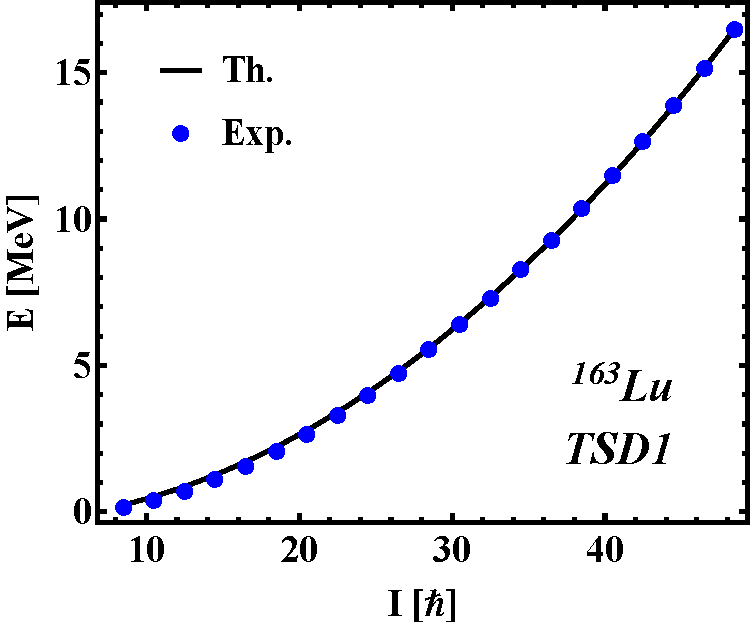
\includegraphics[scale=0.55]{figs/DoubleShift_TSD1.pdf}
\end{minipage}%
\begin{minipage}{.5\textwidth}
  \centering
 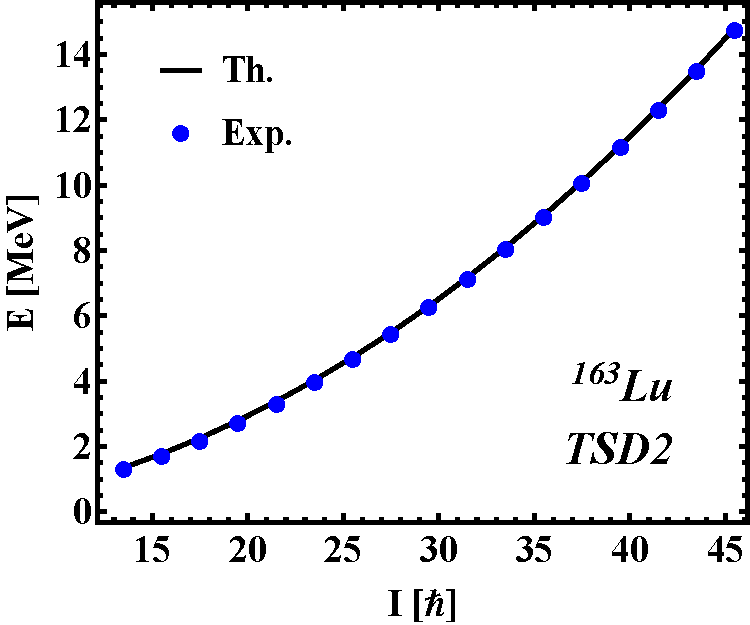
\includegraphics[scale=0.55]{figs/DoubleShift_TSD2.pdf}
\end{minipage}
\caption{Comparison between theoretical and experimental excitation energies for the first two wobbling bands in $^{163}$Lu within the \texttt{W2} model. The theoretical results are obtained with the parameters listed in Table \ref{parameter_set}. Experimental data is taken from \cite{reich2010nuclear}.}
\label{energies-tsd12}
\end{figure}

\begin{figure}
\centering
\begin{minipage}{.5\textwidth}
  \centering
  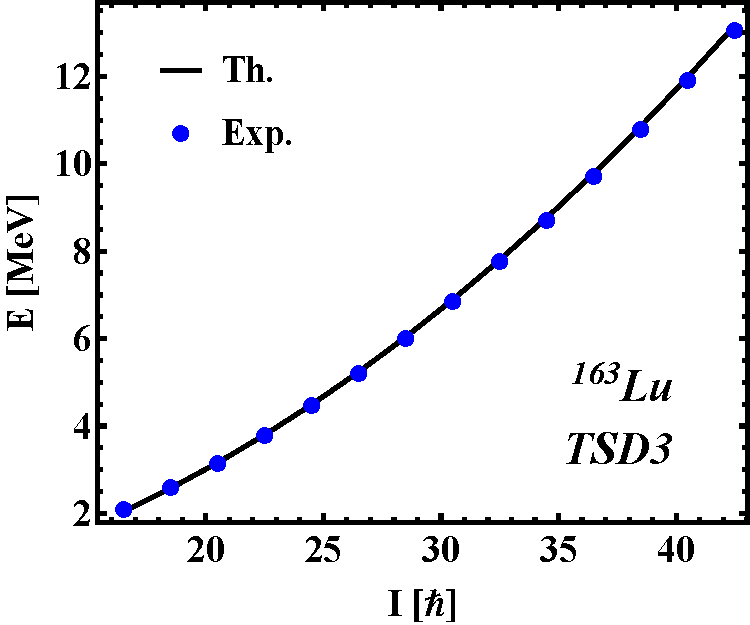
\includegraphics[scale=0.55]{figs/DoubleShift_TSD3.pdf}
\end{minipage}%
\begin{minipage}{.5\textwidth}
  \centering
 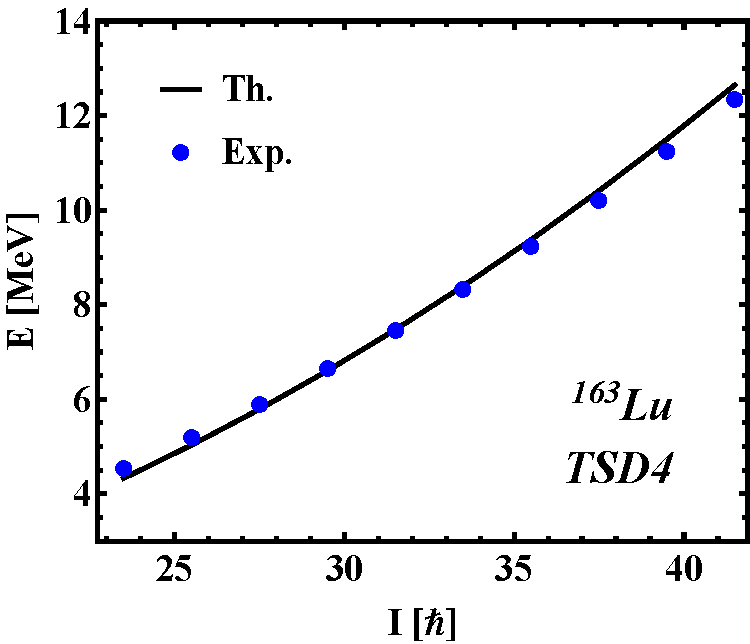
\includegraphics[scale=0.55]{figs/DoubleShift_TSD4.pdf}
\end{minipage}
\caption{Comparison between theoretical and experimental excitation energies for third and fourth wobbling bands in $^{163}$Lu within the \texttt{W2} model. The theoretical results are obtained with the parameters listed in Table \ref{parameter_set}. Experimental data is taken from \cite{reich2010nuclear}.}
    \label{energies-tsd34}
\end{figure}

Another noteworthy aspect of the current formalism is the fact that the difference $\delta_{42}=E_\text{TSD4}^I-E_\text{TSD2}^I$ for all the states has an almost constant value $\delta_{42}\approx0.3\ \text{MeV}$. This suggests that the states of the same a.m. from $TSD_2$ and $TSD_4$ bands might emerge through the parity projection of a sole wave-function that does not have reflection symmetry. In the present case, this is caused by the fact that the wobbling frequency is parity-independent. It is interesting that the action of the parity operator on any rotational state within the angular momentum space will lead to the change of the angular momentum vector from $\vec{I}$ to $-\vec{I}$. Due to this reason, the parity operator commutes with the initial Hamiltonian, and the eigenfunctions of $H$ are characterized by either positive or negative parity (with states of different parities being degenerate). However, one can lift this degeneracy by using an additional linear in the expression $H$. Since in Eq. \ref{prm-hamiltonian} such a linear term is missing, an \emph{ad-hoc} correction of the mean-field with the amount $0.6\ \text{MeV}$ for the states in $TSD_4$ is necessary. As a result, the added shift simulates the breaking of parity symmetry. In contrast to this approach, using a microscopic formalism one starts with a single-particle basis generated by a mean-field without space reflection symmetry, followed by the calculation of the many-body wave-functions (being admixtures of both positive and negative parities). Restoration of the parity symmetry is achieved by selecting from all the wave-functions only the components with a definite parity (projecting the good parity), leading to a doublet structure of positive and negative parity states in the spectrum of $H$. Consequently, the bands $TSD_2$ and $TSD_4$ behave as a pair of parity partners, as defined in \cite{chasman1980incipient,raduta2006description,raduta2006simultaneous}.

% \subsection{Interpretation of the parameter set $\mathcal{P}$}
\subsection{\texorpdfstring{Interpretation of the parameter set $\mathcal{P}$}%
                               {Interpretation of the parameter set P}}\label{results:interpret}

Performing the fitting procedure for the excitation energies of $^{163}$Lu will result in the moments of inertia $\mathcal{I}_k$ that are given in Table \ref{parameter_set}, together with the single-particle potential strength $V$, and triaxiality parameter $\gamma$. Interpretation of their numerical values is mandatory in order to check whether the current formalism is valid or not.

Regarding the moments of inertia, it is clear that the axis of rotation for the energy ellipsoid is the 1-axis, as the largest MOI is $\mathcal{I}_1$, causing a maximal density distribution across this axis \cite{frauendorf2014transverse}. The MOI ordering is $\mathcal{I}_1>\mathcal{I}_2>\mathcal{I}_3$, and compared with the results of the previous work \texttt{W1}, the current 1-axis MOI is bigger than both $\mathcal{I}_1^\text{TSD1,2,3}=63.2\ \hbar^2/\text{MeV}$ and $\mathcal{I}_1^\text{TSD4}=67\ \hbar^2/\text{MeV}$ (data taken from Table 1 in Ref. \cite{raduta2020towards}). This is expected, since here, the $TSD_4$ band is obtained by the coupling of a higher aligned $j$ particle, driving the system to an even larger deformation. One must remember that these are the \emph{effective} MOIs of the entire system, that is the triaxial-rotor + odd-particle. No spin dependence has been inferred for the MOIs, so a possible change in the MOIs ordering with the increase in spin $I$ cannot be studied within the current description. Furthermore, this formalism does not contain microscopic terms, so no presumptions on what causes the obtained MOI ordering can be stated. Although, by working with a quadrupole deformed mean-field, the moments of inertia of the triaxial core should be indeed consistent with the hydrodynamic model. For the sake of completeness, Figure \ref{hydro-mois} shows the evolution of a hydro-dynamical set of MOIs with respect to the triaxiality parameter $\gamma$.

\begin{figure}
\centering
\begin{minipage}{.5\textwidth}
  \centering
  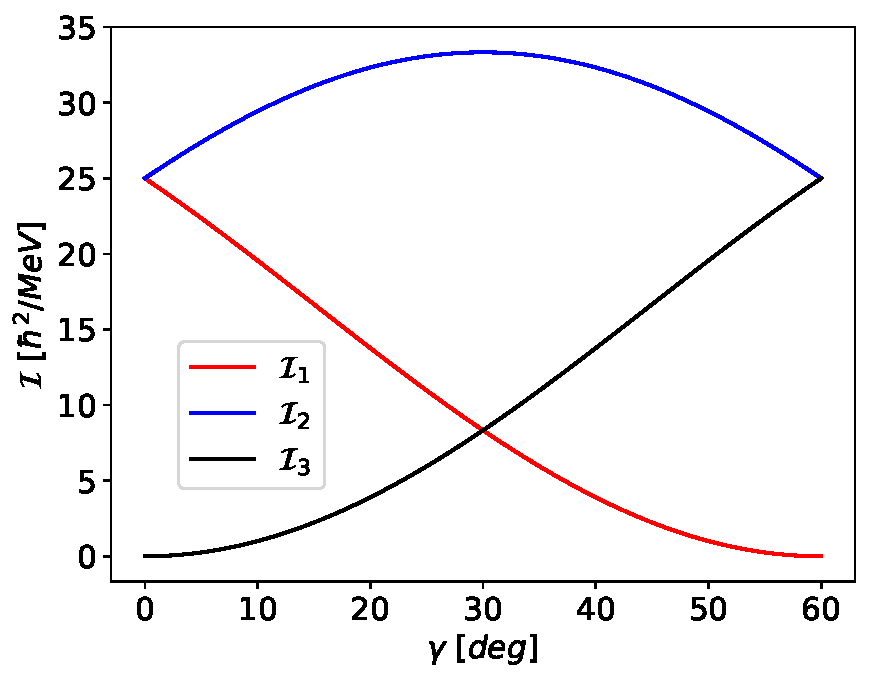
\includegraphics[scale=0.5]{figs/hydro_mois.pdf}
\end{minipage}%
\begin{minipage}{.5\textwidth}
  \centering
 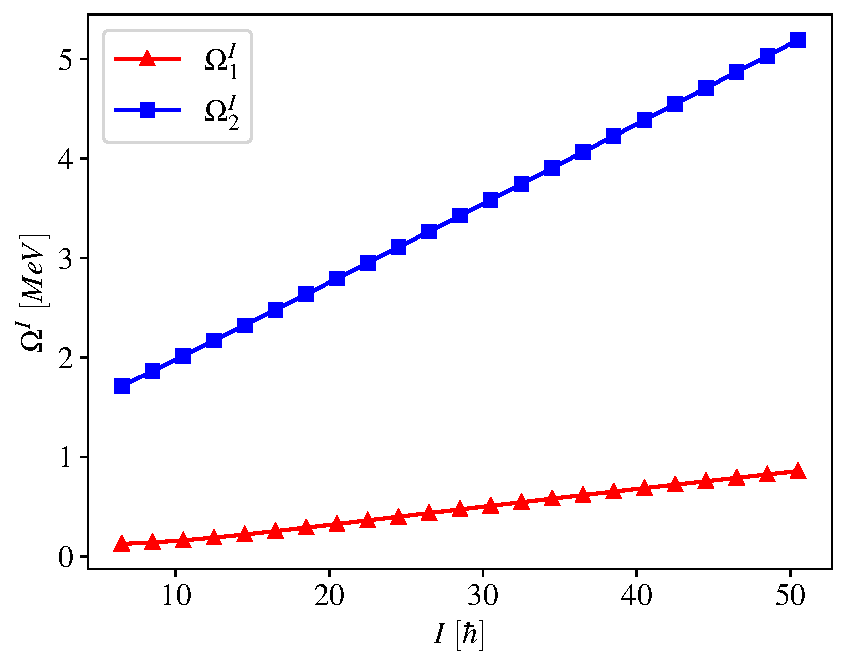
\includegraphics[scale=0.5]{figs/wobbling-frequencies.pdf}
\end{minipage}
\caption{Left-side: The hydrodynamic moments of inertia \cite{tanabe2006algebraic} as function of the triaxiality parameter $\gamma$, for the positive interval $\gamma\in[0^{\circ},60^{\circ}]$, evaluated for a scale factor $\mathcal{I}_0=25\ \text{MeV}^{-1}$. Right-side: The wobbling frequencies defined in Eq. \ref{wobbling-frequencies} as function of total angular momentum, evaluated with the parameter set $\mathcal{P}$ which was obtained through the fitting procedure.}
    \label{hydro-mois}
\end{figure}

Concerning the triaxiality parameter$\gamma$, it has a positive value $\gamma=22^\circ$. This is consistent with the microscopic descriptions based on cranking mechanism for the potential energy surface (PES) of $^{163}$Lu (discussion on PES was done in the previous sections). In fact, the agreement is quite good with the predicted deformed minima of $(\beta_2,\gamma)\approx(0.38,20^\circ)$ \cite{jensen2002wobbling,jensen2004coexisting}. Comparing the current \texttt{W2} model with already existing descriptions which take $\gamma$ to be fixed a-priori throughout the calculations (e.g., \cite{tanabe2006algebraic,tanabe2017stability}), here $\gamma$ is obtained through the fitting process in a self-consistent manner. Moreover, its value is slightly larger than the one obtained in \texttt{W1} formalism ($\gamma=17^\circ$). This might be due to the larger ratios $\mathcal{I}_1/\mathcal{I}_{2,3}$, which in the present case they appear to be bigger ($\mathcal{I}_1/\mathcal{I}_{2}\approx4.8$ for \texttt{W2}, compared to $\approx3.2$ in the previous approach \text{W1}).

Finally, the single-particle potential strength, which causes the odd-proton to move in the quadrupole deformed mean-field, has a value of $V=2.1\ \text{MeV}$. In \texttt{W1}, this parameter was $V^{\text{TSD1,2,3}}=3.1\ \text{MeV}$ and $V^\text{TSD4}=0.7\ \text{MeV}$. An explanation for its decrease in the present case might be due to the upward shift in the energy caused by the un-favored partner, or due to the energetic shift of the parity partner, indicating a quenching effect on the quadrupole deformation of the triaxial system. Nevertheless, the obtained value seems to be consistent with the previous calculations, the current value of $V$ being close to the average value of $V$'s from $\texttt{W1}$. Other interpretations \cite{tanabe2017stability} that were developed using a similar single-particle potential term in the Hamiltonian adopted values of around $V=1.6\ \text{MeV}$, however, that was for an isotope with smaller quadrupole deformation $\beta_2=0.18$. Interesting research using a single-$j$ shell model which was aimed at obtaining a realistic expression for the deformation parameter has been performed in \cite{shou2009coupling}. Therein, results for the potential strength of odd-$A$ nuclei with similar mass, but different quasiparticle configurations were numerically obtained. Adoption of an equivalent description for the odd-$j$ particle within \texttt{W2} could be done, and then compare results for a corresponding configuration. This could be the motivating factor for future work. Concluding this subsection, the obtained values of $\mathcal{P}$ seem to not only describe the wobbling spectrum of $^{163}$Lu very well (see results in Figures \ref{energies-tsd12} and \ref{energies-tsd34}), but they are also consistent with the previous formalism \texttt{W1}, or even with other interpretations from the literature. 


\begin{table}[h!t]%
\caption{This table is taken from RJP volume \textbf{50}(1-2) from page 43 (2005). It gives the ``
\textit{number of bound states dependence on the radius of space curvature for $\alpha = 0.005$, $U_0 = 1$}''.}
\centering
\begin{tabular}{|c|c|}
\hline
Value $\rho$ & Value $\varepsilon$ \cr
\hline
$\rho = 50$ & -- \cr
$\rho = 100$ & -- \cr
$\rho = 250$ & $\varepsilon_1 = 0.0289$ \cr
$\rho = 400$ & $\varepsilon_1 = 0.3772$ \cr
$\rho = 1000$ & $\varepsilon_1 = 0.4142$, $\varepsilon_2 = 0.8495$ \cr
\hline
\end{tabular}
\label{table1}
\end{table}


\begin{acknowledgement}
The author(s) would like to dedicate this at the Romanian Academy Publishing House.
\end{acknowledgement}


\begin{thebibliography}{99}
\bibitem{knuth}D. E. Knuth, D. R. Bibby, ``\textit{The \TeX book}'', 20th edn. (AMS \& Addison-Wesley Publ. Co., 1991).
\bibitem{dknuthhp} D. E. Knuth homepage: \href{http://www-cs-faculty.stanford.edu/~knuth/}{\small\ttfamily www-cs-faculty.stanford.edu/\~{}knuth}.

\end{thebibliography}


\end{document}